\chapter{Opis eksperymentu}
\section{Układ pomiarowy}
Układ pomiarowt składał się z:
\begin{itemize}
\item Komputera z systemem Linux (Ubuntu) --- wymagane jest, aby na komputerze zainstalowany był język Python wraz z bibliotekami:
matplotlib, numpy, PyQt5. Do sterowania sprzętem przy pomocy programów opisanych w 3 rozdziale wymagane są uprawnienia administratora.
\item Zasilacza diod laserowych firmy Thorlabs model LDC4005~\cite{Ldc_book}--- zapewnia stabilne zasilanie prądowe lasera prądem do 5\,A.
Możliwe jest zasilanie ciągłe i impulsowe. Posiada interfejsem SCPI~\cite{Ldc_book_prog}, umożliwiający sterowanie za pomocą komputera przez USB.
\item Miernik mocy firmy Thorlas firmy Thorlabs model PM100~\cite{Pm100_book} --- stworzony do mierzenia mocy wyjściowej z lasera. Pozwala operować na
długościach fali od 400\,nm do 1100\,nm. Posiada interfejsem SCPI~\cite{Pm100_book}, umożliwiający sterowanie za pomocą komputera przez USB.
\item Kontroler temperatury diod laserowych firmy Thorlabs--- precyzyjny kontroler temperatury pozwalający na zmiany temperatury
chłodniczy lasera podczas operowania prądami do 2\,A.
\end{itemize}
\subsection{Przebieg pomiarów}
Laser był umieszczony w mocowaniu stabilizującym temperaturę diod laserowych połączony z zasilaczem diod laserowych oraz kontrolerem temperatury.
Na wyjściu lasera umieszczony był miernik mocy. Komunikacja z zasilaczem oraz miernikiem odbywała się za pomocą standardu
komend SCPI przez połączenie USB przez wykorzystanie programów opisanych w rozdziale 3.
Temperatura była zmieniana manualnie na kontrolerze temperatury.
Charakterystyki wyjściowe (czyli wartości prądu zasilania, napięcia na laserze oraz mocy wyjściowej)
mierzone były przy pomocy zasilania ciągłego. Wyniki zapisywane były w pliku tekstowym. Schematyczny rysunek układu pomiarowego przedstawiony jest
na rysunku 5.1.
\begin{figure}
\center
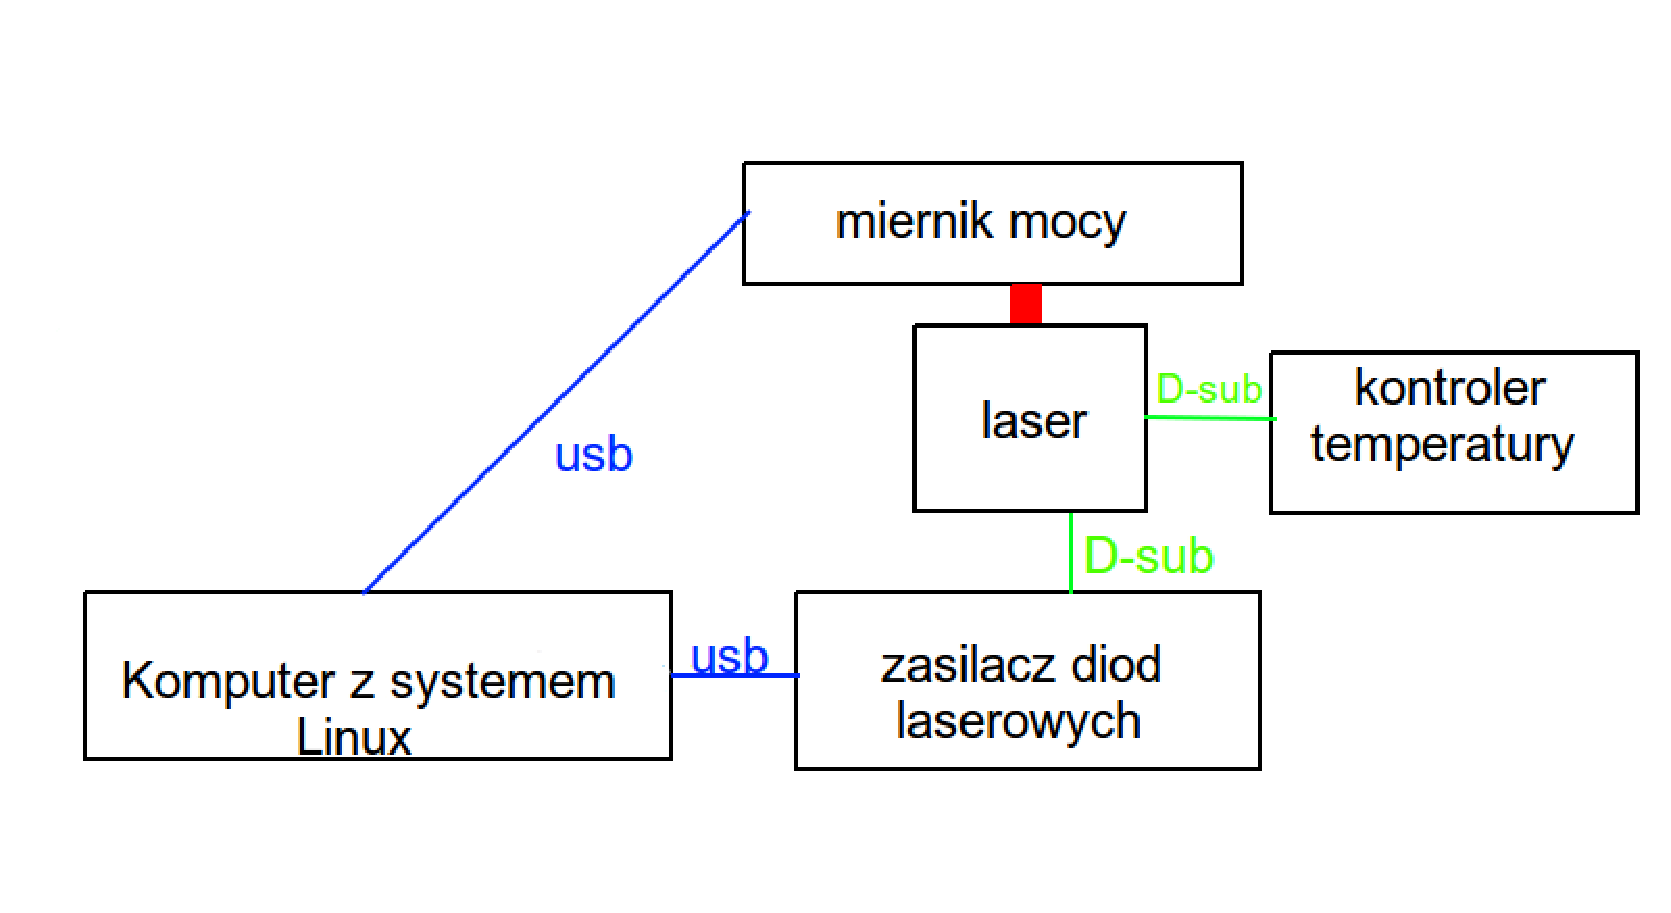
\includegraphics[scale=0.35]{schemat.eps}
\label{fig:sch_pom}
\caption{Schemat układu pomiarowego.}
\end{figure}